
%%
%% Template chap2.tex
%%

\chapter{Results and Discussion}
\label{cha:results}

The dataset

\begin{figure}[p]
	\centering
	\begin{subfigure}{\textwidth}
		\centering
		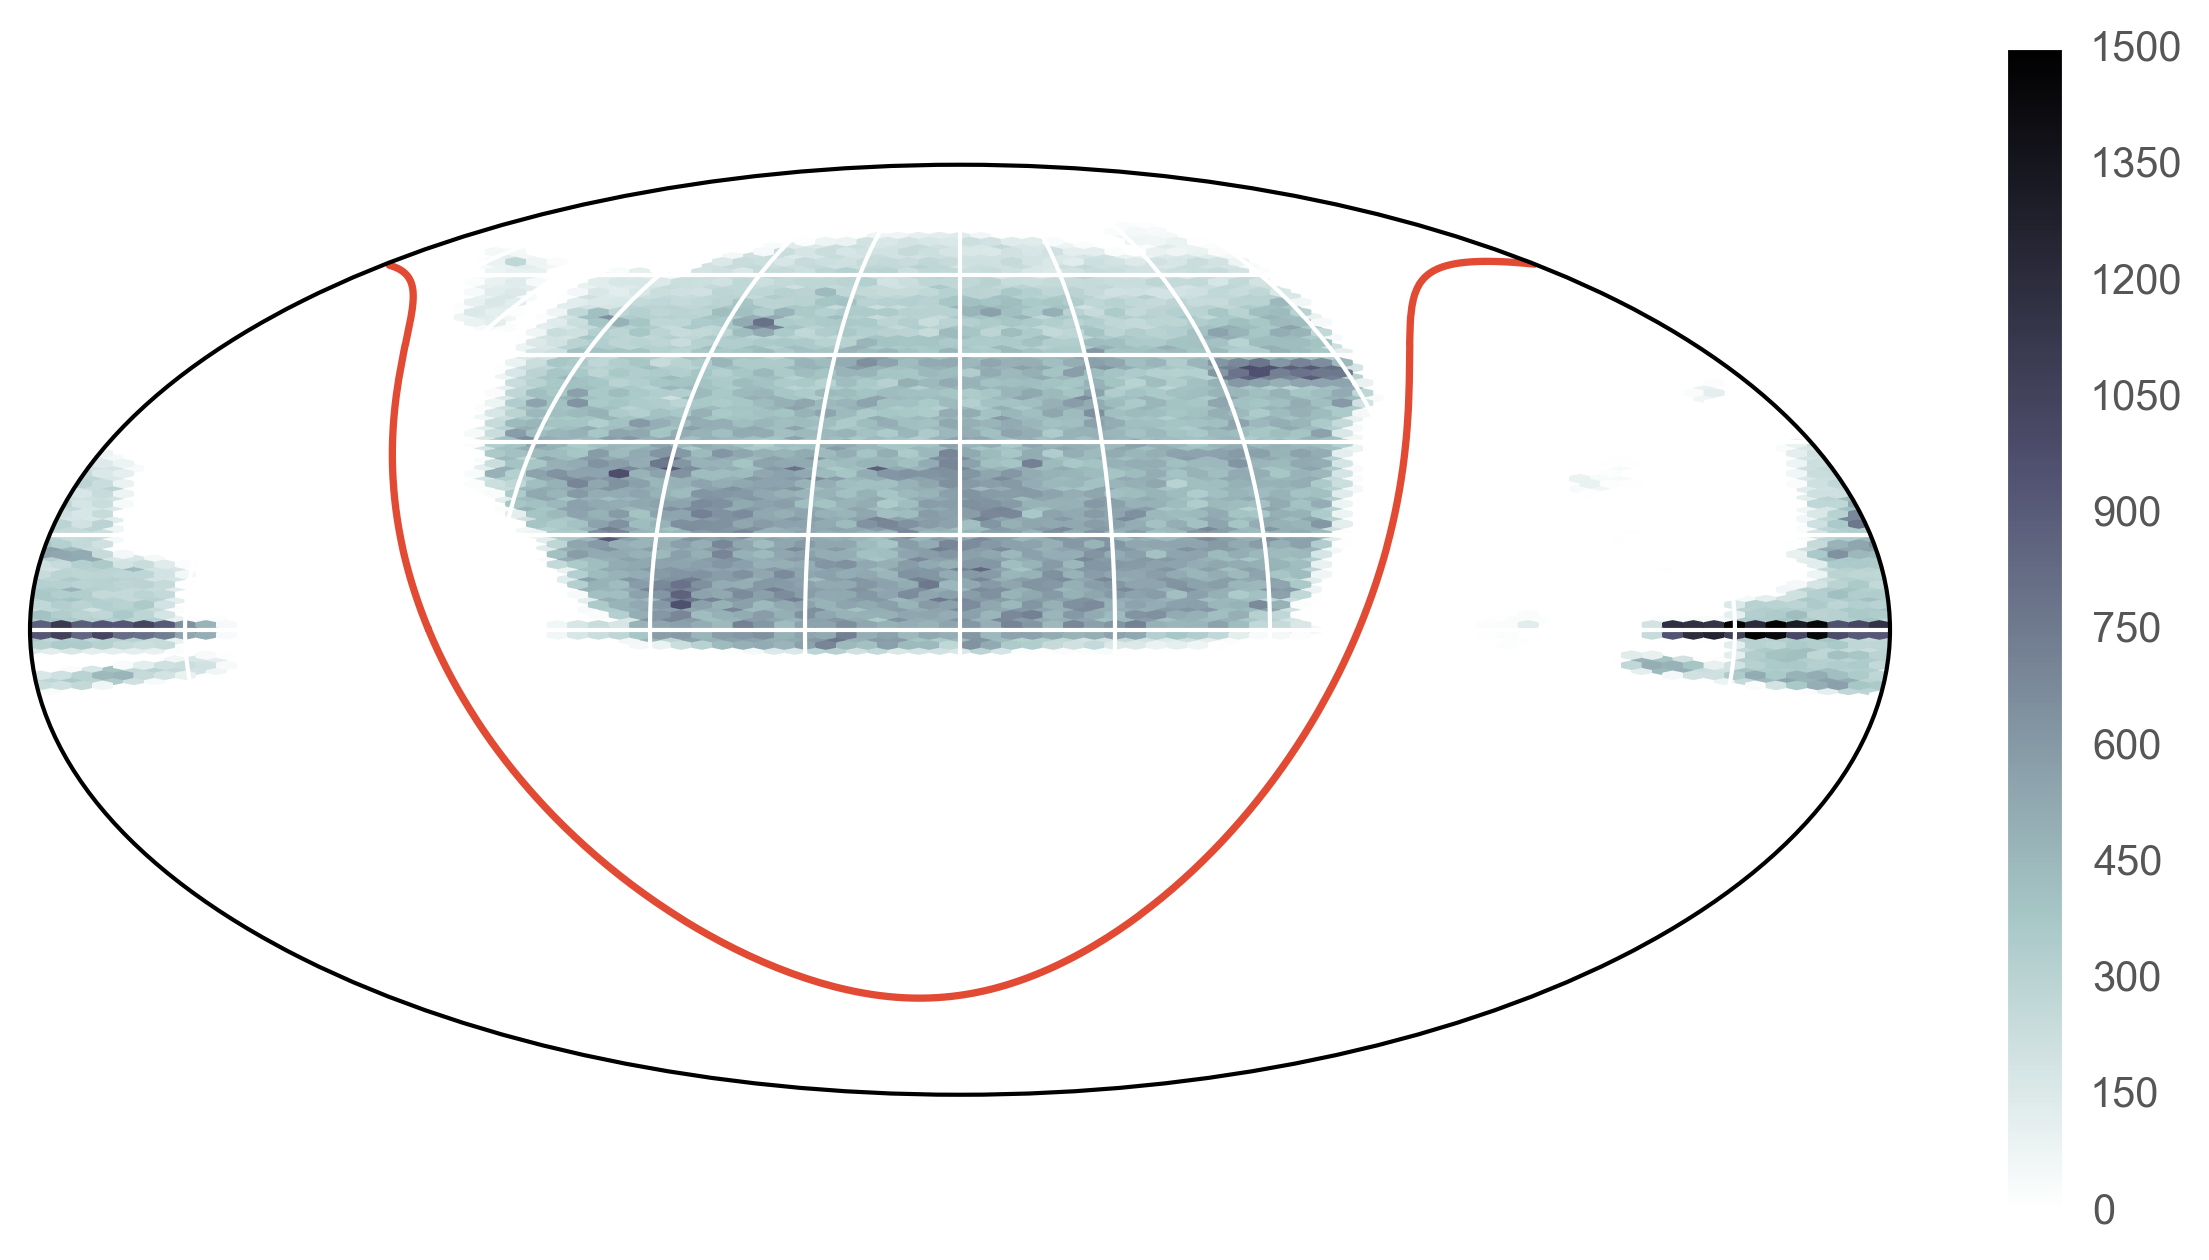
\includegraphics[width=0.75\textwidth]{figures/map_train_galaxies}
		\caption{Distribution of galaxies.}
		\label{fig:orbit1}
	\end{subfigure}\\
	\begin{subfigure}{\textwidth}
		\centering
		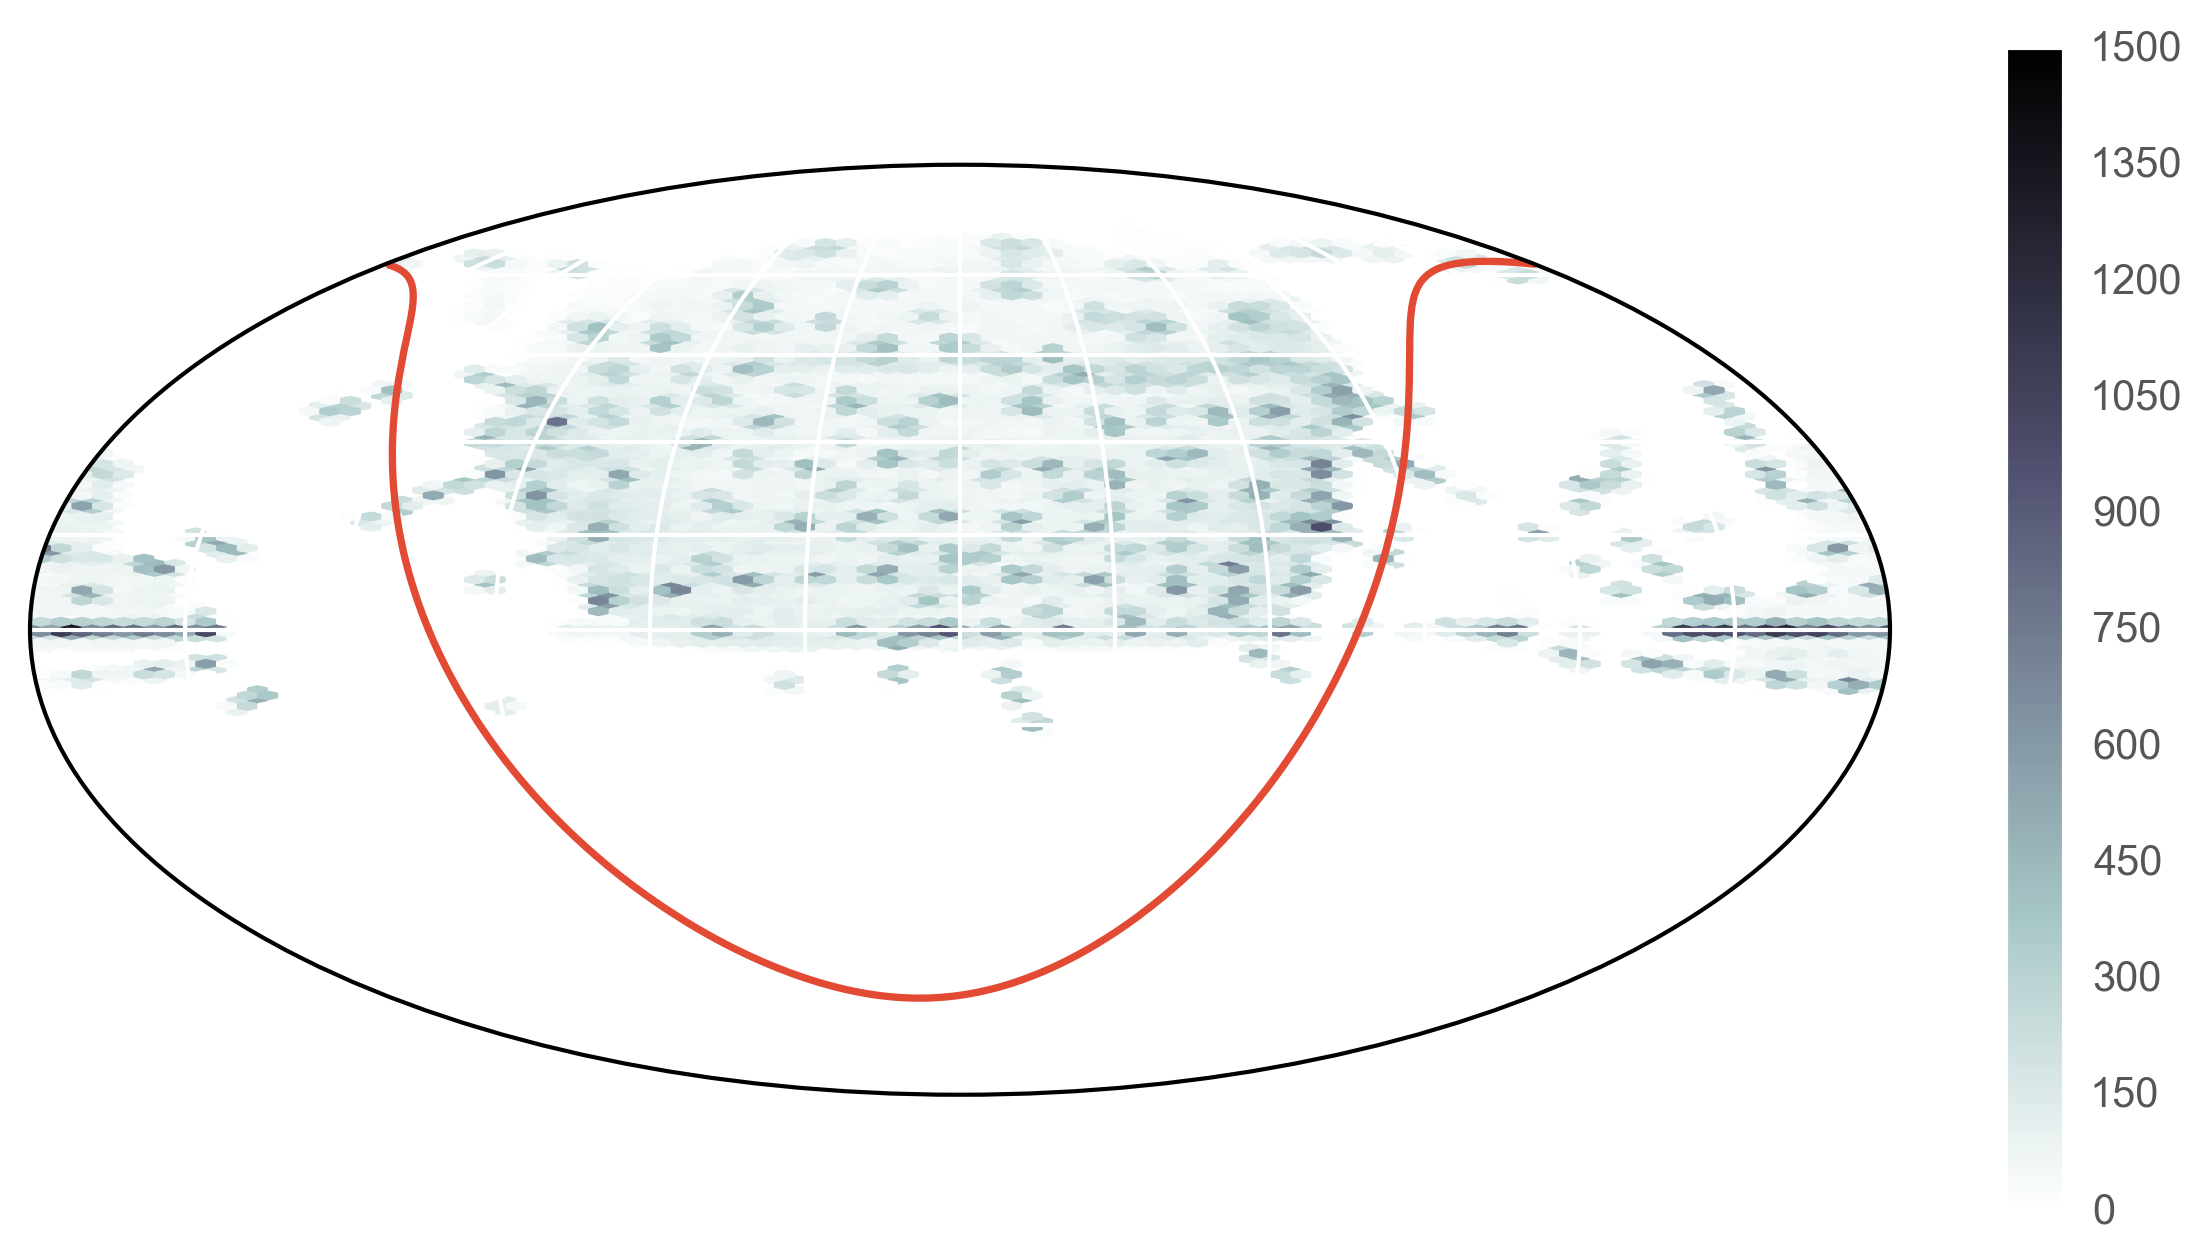
\includegraphics[width=0.75\linewidth]{figures/map_train_stars}
		\caption{Distribution of stars.}
		\label{fig:orbit2}
	\end{subfigure}
	\begin{subfigure}{\textwidth}
		\centering
		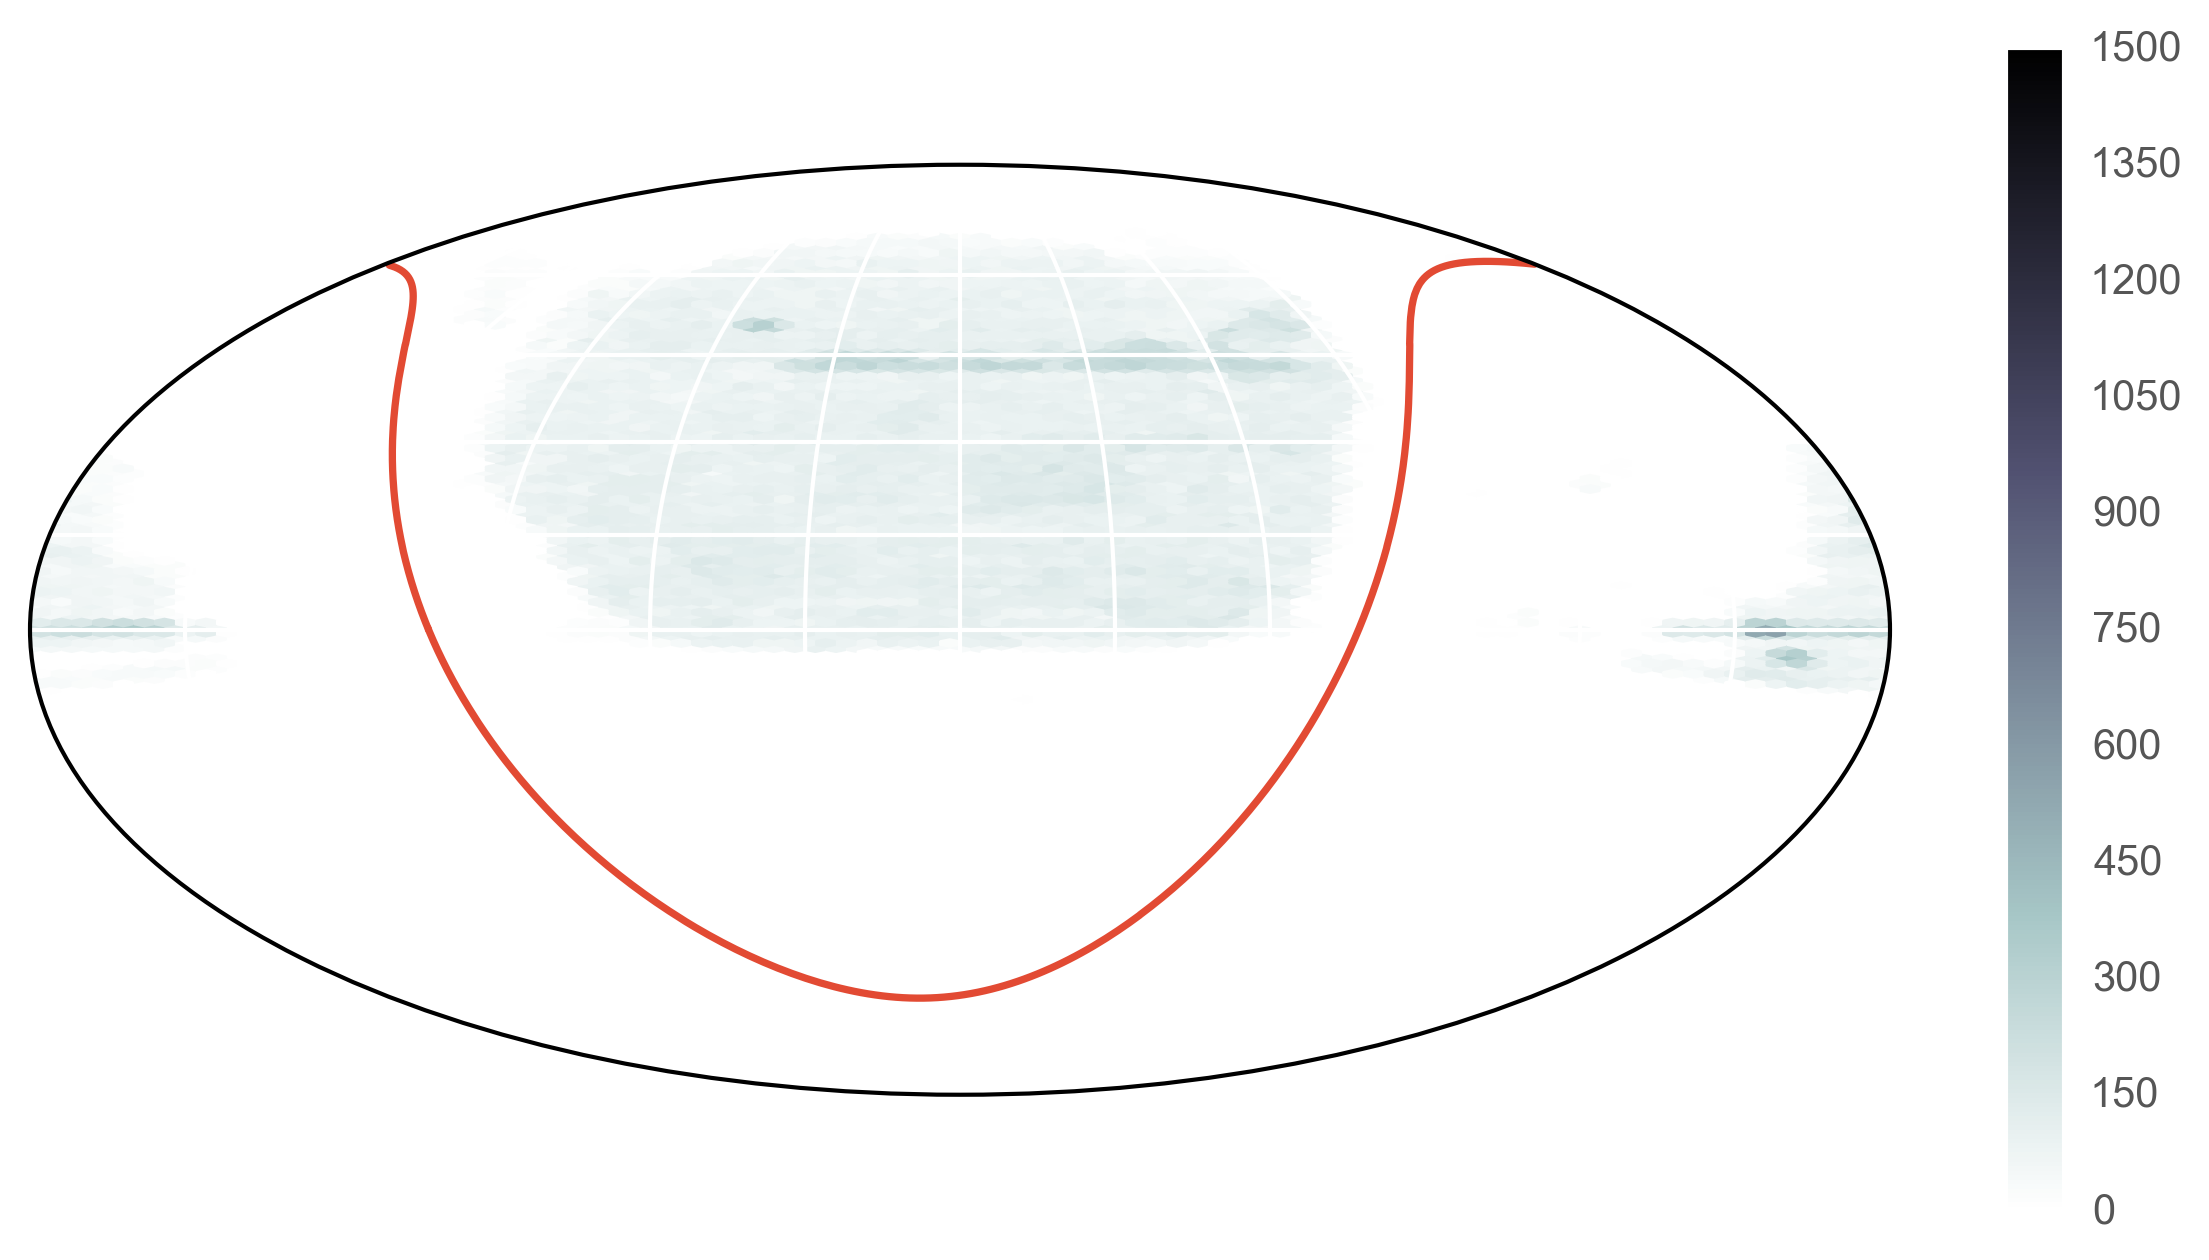
\includegraphics[width=0.75\linewidth]{figures/map_train_quasars}
		\caption{Distribution of quasars.}
		\label{fig:orbit3}
	\end{subfigure}
	\caption{Distribution of the classes in the training set.}
	\label{fig:orbit}
\end{figure}


Learning curve with random sampling.


\begin{figure}[h]
	\centering
	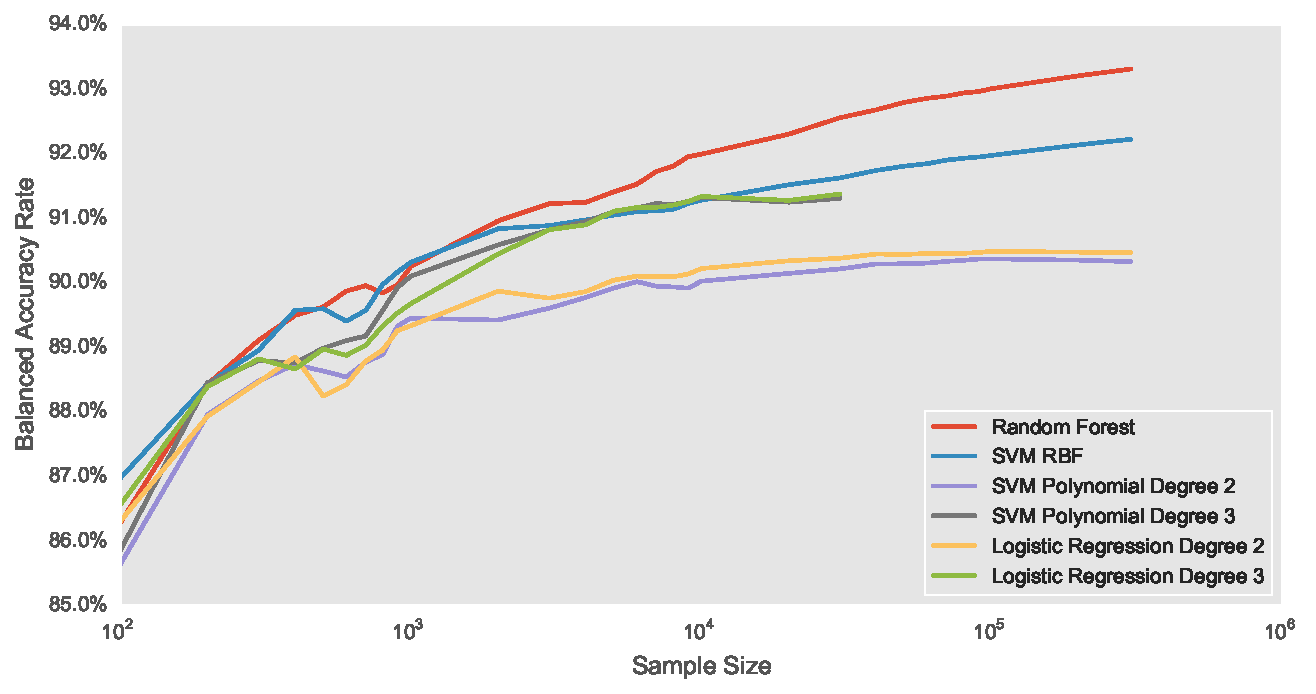
\includegraphics[width=\textwidth]{figures/learning_curves}
	\caption{Learning curves.}
	\label{fig:learning}
\end{figure}



\section{Active Learning Results}
\label{sec:results1}

\section{Some More Results}
\label{sec:results2}

%%% Local Variables: 
%%% mode: latex
%%% TeX-master: "thesis"
%%% End: 
